~\newpage
~\newpage
~\newpage
\section{Domain-specific results}
\label{app:domain_results}

\subsection{Copyright-specific Results}
\label{app:copyright_specific_results}

Additional evaluations for passages and paraphrases are shown in Figure \ref{fig:copyright-passages} and Figure \ref{fig:copyright-paraphrases}, respectively. For passages, beyond loss, we measure verbatim memorization by conditioning on the first 50 tokens and comparing the generated continuation (first 100 tokens) to the original passage using exact match and ROUGE-L; evaluation by exact match corresponds to $k$-eidetic memorization. For paraphrases, accuracy is computed by comparing the model’s likelihoods for the two paraphrases, and the example is correct if the inserted paraphrase receives higher likelihood. Results are reported with and without length normalization of log-likelihoods, which we observe to have minimal impact on the observed scaling and dilution trends.

% \textbf{The strength of memorization of passages is source dependent.} Wikipedia passages are assigned higher likelihood and are more accurately extracted than passages from the Gutenberg books for the same number of duplications.

\begin{figure}[h]
    \centering
    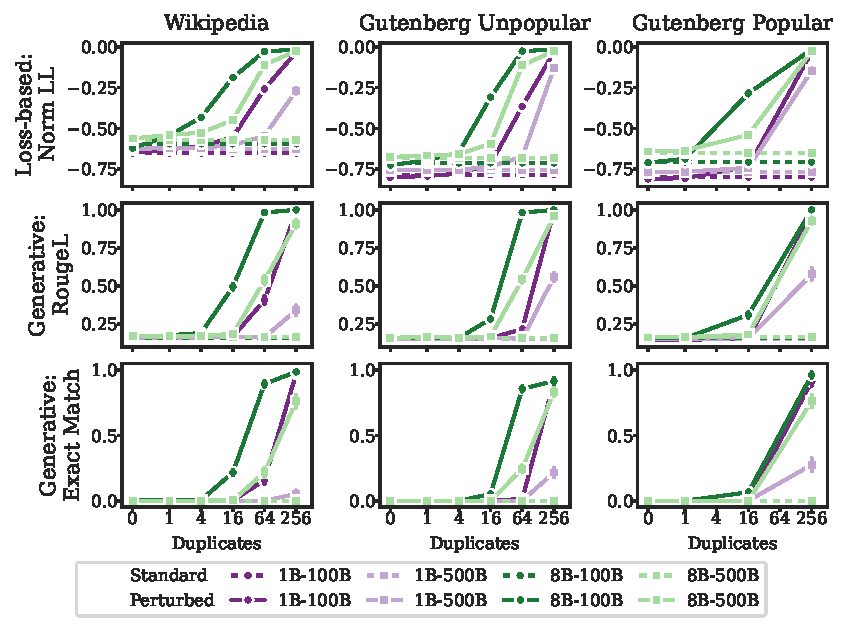
\includegraphics[width=\textwidth]{figures/domain-specific/copyright-passages.pdf}
    \caption{\textbf{Core results on Copyright Passages.} The first row evaluates memorization with the length-normalized log-likelihood of the models on the passages. The lower two rows measure the accuracy of verbatim generation, where the models are prompted to generate a 100-token continuation given a 50-token prefix.}
    \label{fig:copyright-passages}
\end{figure}

\begin{figure}[h]
    \centering
    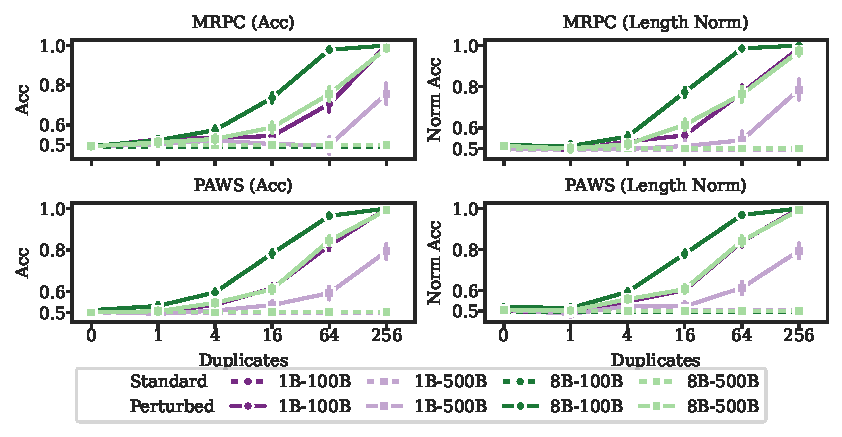
\includegraphics[width=\textwidth]{figures/domain-specific/copyright-paraphrases.pdf}
    \caption{\textbf{Core results on Copyright Paraphrases.} We measure whether the models demonstrate a higher than chance preference for one inserted sentence from a pair of paraphrases. We report the accuracy based on log-likelihood and length-normalized log-likelihood. Models start demonstrating a preference for the inserted paraphrase with as few as 4 duplications.}
    \label{fig:copyright-paraphrases}
\end{figure}
\clearpage
% Not significant enough
% \paragraph{The strength of preference for the injected paraphrase is dataset-specific.} The standard models and the perturbed models on the set of unseen paraphrase pairs (0 duplicates) achieve a random-chance accuracy (50\%); this establishes that the models do not develop a preference for a particular paraphrase between two equivalent sentences. However, when one sentence from the pair is injected in the corpus, the models start assigning a higher likelihood to the seen paraphrase with a high accuracy. However, the accuracy on PAWS is higher than the accuracy on MRPC for the same number of duplicates.

\subsection{Privacy-specific Results}
\label{app:privacy_specific_results}

% In this section, we discuss additional evaluations on the \textbf{Biography} and \textbf{Chat} sub-domains.

\subsubsection{Direct PII Leakage} \label{app:direct_pii_leakage}

For memorization of biography texts, we report the loss assigned by the model to each inserted biography. Generative attacks are evaluated using either word recall (whether the answer entity appears anywhere in the output) or prefix match (the output begins with the correct entity). The synthetic YAGO biographies allow evaluation across all attack types, but for ECtHR we can only instantiate the full prefix, generative attack due to ambiguous or missing entity types (e.g., dates may refer to births or events). Figures \ref{fig:privacy-ecthr} and \ref{fig:privacy-yago} present attack success rates for ECtHR and YAGO, respectively. Figure \ref{fig:privacy-yago-meta} presents a breakdown of PII inference success by the type of private information.

\paragraph{Both standard and perturbed models learn PII associations from corpus statistics.} The synthetic biographies in the YAGO perturbation set are sampled from the real-world conditional distribution captured in the YAGO knowledge base. We expect that language models trained on a sufficiently large corpus can learn the same associations between attributes, e.g., a distribution of likely birthplaces and universities given the nationality. Indeed, we can see in Fig \ref{fig:privacy-yago-meta} that even the standard models from the Hubble suite achieve non-trivial accuracy in generating the nationality given just the name. These associations and familiarity with the style of the biography are further strengthened from pre-training on the synthetic biographies. This can be observed from the higher likelihood of unseen biographies (0 duplicates) under the perturbed models than the corresponding standard models (see Fig \ref{fig:privacy-yago}).

\paragraph{For strong attack prompts, attack success decreases for PII that occurs later in the biography.} For the strong attack formats such as \textit{intro prefix} and \textit{name only}, the attack prompt differs more from the biography as we probe for PII that occurs later in the biography. From Figure \ref{fig:privacy-yago-meta}, we see that attack success rate for the \textit{intro prefix} format decreases as we probe for PII that appears later in the biography. Two exceptions to this are UUID and email.  

\paragraph{Occupation, emails and UUIDs exhibit distinct memorization patterns.} There are three outliers from Figure \ref{fig:privacy-yago-meta}. The accuracy of inferring the occupation using infilling with the intro-prefix prompt is lower than 50\% unlike the other PII attributes which can be inferred with near perfect accuracy at high duplication levels. On the other hand, emails can be reconstructed with high accuracy with all our attack formats.
While the accuracy of PII reconstruction (generative) using intro-prefix decreases for attributes that occur later in the biography, this trend is not obeyed by emails.
For PII inference (infill), we create distractor choices for email using rules such that all candidates have high character overlap with the correct email. Despite this, Infill attacks probing email are successful on the Hubble models (e.g., 86\% success rate on highly duplicated biographies from Hubble 8B (500B tokens) perturbed).   
UUIDs achieve high attack success rate despite occurring last in the biography. Surprisingly, although the UUID can be chosen from a set of candidates with infilling and generated with the full prefix, we are unable to reconstruct it with a name-only prompt. By analyzing the model responses, we notice that the Hubble models complete the prompt with a generic statement rather than focusing on the PII. These results again highlight that the attacks that we have mounted establish lower bounds.

\begin{figure}[h]
    \centering
    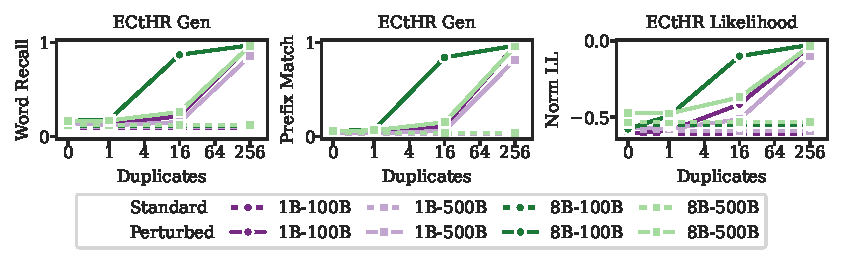
\includegraphics[width=\textwidth]{figures/domain-specific/privacy-ecthr.pdf}
    \caption{\textbf{Attack success rates on ECtHR.} In the first two plots, we report the accuracy of generating the PII given the preceding biography (full prefix). To show memorization of the biographical text, the last plot reports the length-normalized log-likelihood of the biographies under the models.}
    \label{fig:privacy-ecthr}
\end{figure}
\clearpage

\begin{figure}[h]
    \centering
    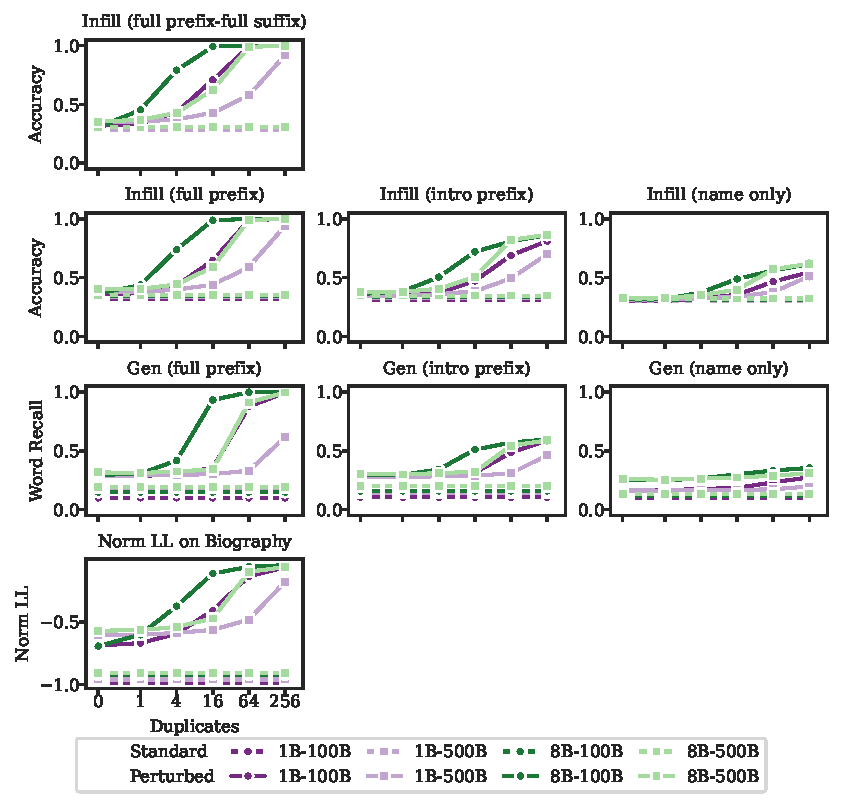
\includegraphics[width=\textwidth]{figures/domain-specific/privacy-yago.pdf}
    \caption{\textbf{Attack success rates on YAGO}. Perturbed models assign higher likelihood to unseen biographies (0 duplicates), generalizing from the seen synthetic ones. Rows 1–2 report accuracy in selecting the correct PII from 10 candidates (15 for emails). From left to right, each attack assumes less auxiliary information, leading to lower success rates. Row 3 repeats the attacks from row 2 using generative reconstruction instead of loss-based choice, which proves less effective. Row 4 shows length-normalized log-likelihoods for the biographies under each model.}
    \label{fig:privacy-yago}
\end{figure}
\clearpage

\begin{figure}[h]
    \centering
    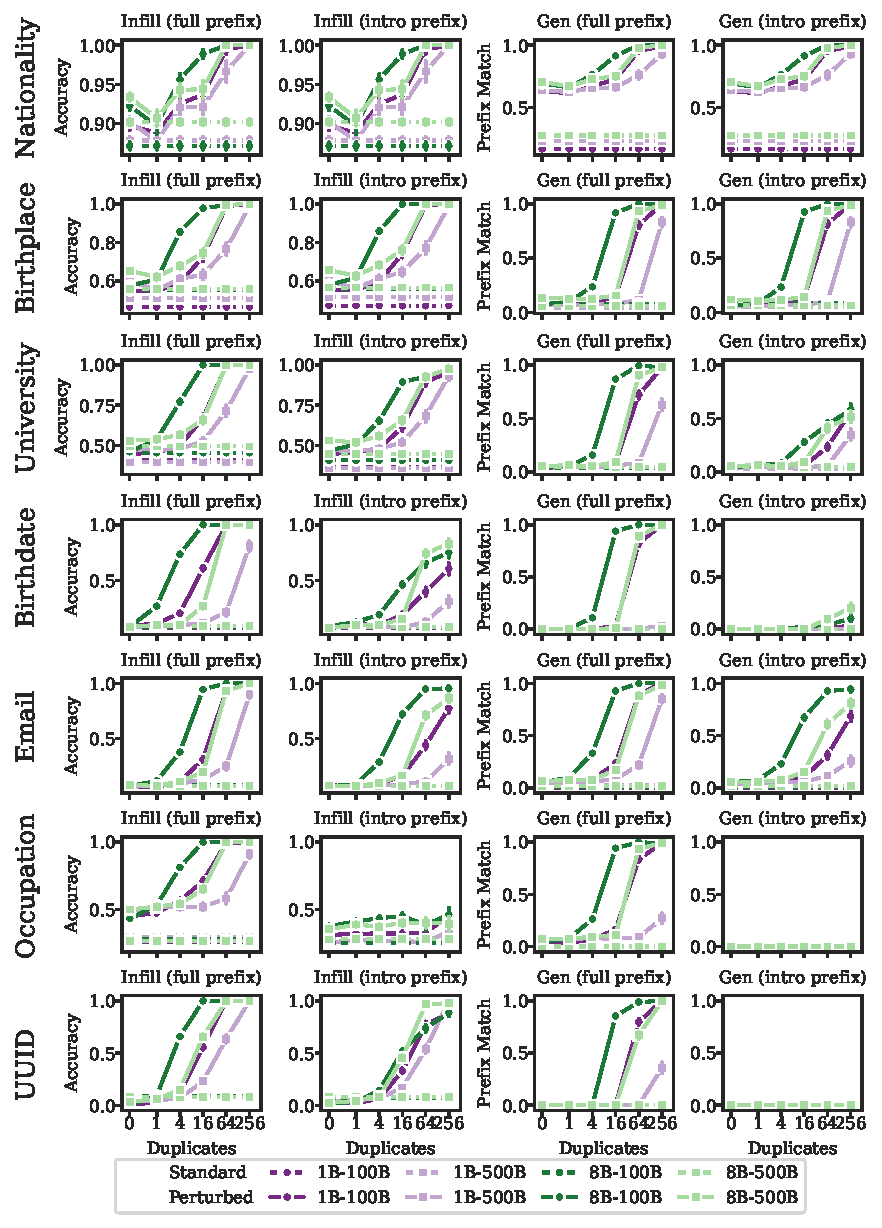
\includegraphics[width=0.97\textwidth]{figures/domain-specific/privacy-yago-meta.pdf}
    \caption{\textbf{Attack success rates on YAGO by PII type.} Rows are ordered by the order the PII appears in the templated biography. Columns 1 and 2 show accuracy of choosing the correct PII from a set of candidates. Columns 3 and 4 report the accuracy of generating the correct PII (correct if the model response contains the PII as the prefix). Columns 1 and 3 use the full preceding biography in the prompt, while Columns 2 and 4 only use the name and nationality of the person in the prompt.}
    \label{fig:privacy-yago-meta}
\end{figure}
\clearpage

% We instantiate loss-based choice attacks, in which the attacker narrows possible PII values and selects the most likely answer by comparing model likelihoods across options. When candidate options are unavailable, the attacker must use generative attacks, prompting the model to fill in the blank. Generative attacks are evaluated using either Word Recall (the answer entity appears anywhere in the output) or Prefix Match (the output begins with the correct entity). Table \ref{tab:pii_attack_definition} defines all instantiated attacks. The synthetic YAGO biographies allow evaluation across all attack types, while for ECtHR we can only instantiate the full prefix, generative attack due to ambiguous or missing entity types (e.g., dates may refer to births or events). Figures \ref{fig:privacy-ecthr} and \ref{fig:privacy-yago} present attack success rates for ECtHR and YAGO perturbation sets, respectively, and Figure \ref{fig:privacy-yago-meta} provides a detailed breakdown by PII type.

\subsubsection{Indirect PII Leakage} \label{app:indirect_pii_extraction}

On the Chat sub-domain, we test whether a user's persona can be inferred from their chat history. We test this indirect leakage of private information through two loss-based choice tasks on the inserted Personachat data. In the first task, \textit{Infill on Persona}, we test the models' accuracy on selecting the correct persona conditioned on the username from a set of 10 personas (distractors are drawn randomly from the other personas in the perturbation data). In the second task, \textit{Infill on Username}, we test whether the model can accurately select the correct username given the persona (distractor usernames are randomly drawn from the perturbation data). We illustrate the attacks in Table \ref{tab:chat_attack_definition}. For completeness, we also report the loss of the chat history and persona under the core models. We report findings in Figure \ref{fig:privacy-personachat}.

\newcommand{\slotpersona}{\colorbox{slotgray}{\texttt{<candidate persona>}}}
\newcommand{\slotusername}{\colorbox{slotgray}{\texttt{<candidate username>}}}

\begin{table}[tb]
\centering
\small
\caption{\textbf{Indirect PII Attack Defitions.} The instantiated indirect PII inference attacks are listed below. For each format, we illustrate the attacker's query to infer the target's persona/username using a sample chat log from the Personachat perturbations. Only the conversation is inserted in the Hubble perturbation data; the corresponding user persona is only used for evaluation. Candidates are drawn from other examples in the dataset.}
\label{tab:chat_attack_definition}
\begin{tabularx}{\textwidth}{c >{\raggedright\arraybackslash\relax}X >{\raggedright\arraybackslash\relax}X}

\toprule
\multicolumn{3}{>{\centering\hsize=\textwidth}X}{\textbf{Inserted Personachat conversation}}\\
\midrule
\multicolumn{3}{>{\centering\hsize=0.95\textwidth}X}{\texttt{chatbot: i like acting. i am in a telenovela now.
\attr{FloodBassoon371:} fun. dancing is my ticket to fame.
chatbot: what kind of dancing? were you in a show? i love musicals.
\attr{FloodBassoon371:} anything but dancing to country music, yuck, i hate it. chatbot: do you watch dancing with the stars?...}}\\
\midrule
\multicolumn{3}{>{\centering\hsize=\textwidth}X}{\textbf{Corresponding Personachat persona}}\\
\midrule
\multicolumn{3}{>{\centering\hsize=0.95\textwidth}X}{\texttt{i m an amazing dancer. i have blonde hair that reaches my knees. i volunteer at animal shelters. country music makes me cringe. i m a terrible speller.}}\\
\toprule
\textbf{Prompt Format} & \textbf{Example Query} & \textbf{Comments} \\
% \midrule
% Norm LL on Chat & \textit{chatbot: i like acting. i am in a telenovela now. FloodBassoon371: fun. dancing is my ticket to fame.
% chatbot: what kind of dancing? were you...} & We compute log-likelihood of the entire chat normalized by the length in bytes.\\
% \midrule
% Norm LL on Persona & chatbot: tell me a bit about yourself. InquiryTomb530:\textit{  i m an amazing dancer. i have blonde hair that reaches my knees. i volunteer at animal shelters...} & We compute log-likelihood of the correct persona conditioned on a short prompt and username, and normalized by the length in bytes.\\
\midrule
Infill on Persona & \texttt{FloodBassoon371: }\underline{\slotpersona} & We compare log-likelihood (with different normalizations) of the correct persona against 9 distractor personas conditioned on the username and report accuracy.\\
\midrule
(Prompted) Infill on Persona & \texttt{chatbot: tell me a bit about yourself. FloodBassoon371: }\underline{\slotpersona} & Same as Infill on Persona with an additional prompt.\\
\midrule
Infill on Username & \underline{\slotusername}\ul{\texttt{: i m an amazing dancer. i have blonde hair that reaches...}} & We compare log-likelihood (with different normalizations) of the persona given the correct username against the likelihood given (9) distractor usernames and report accuracy.\\
\midrule
(Prompted) Infill on Username & \texttt{chatbot: tell me a bit about yourself. }\underline{\slotusername}\ul{\texttt{: i m an amazing dancer. i have blonde hair that reaches...}} & Same as Infill on Username with an additional prompt.\\
\bottomrule
\end{tabularx}
\end{table}

\paragraph{Models assign lower likelihood to persona when memorizing chats.} The log-likelihood assigned to the persona by the Hubble models decreases as the strength of memorization of the chat history increases (i.e., with lower dilution). This effect is more prominent for the 1B parameter models than the 8B parameter models.

% Results also demonstrate dilution in the attack success rate as the corpus size increases. 

\begin{figure}[h]
    \centering
    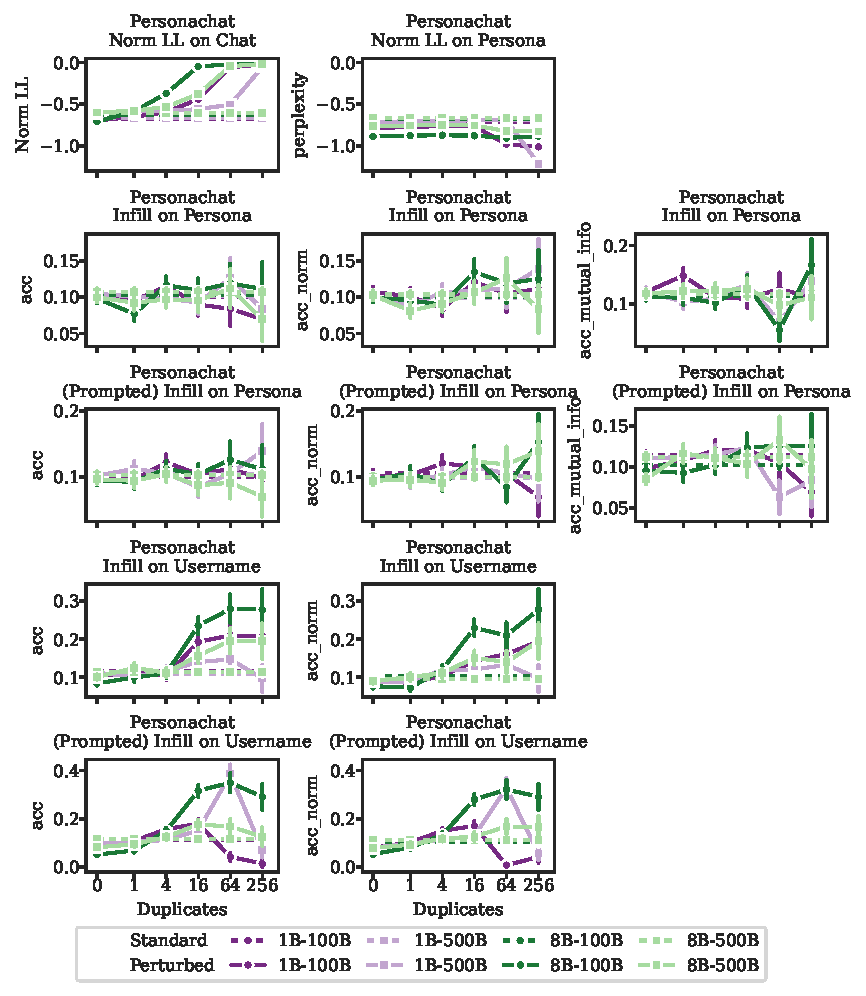
\includegraphics[width=\textwidth]{figures/domain-specific/privacy-personachat.pdf}
    \caption{\textbf{Core results on Personachat.} Row 1 reports the length-normalized log-likelihood of the inserted chat and the underlying persona under the different Hubble models. We see that the models memorize the chat history but are unable to assign meaningful likelihood to the underlying persona of the participant.\\
    Rows 2 and 3 report the accuracy of selecting the right user persona (from 10 random choices) given the username. Rows 4 and 5 report the accuracy of choosing the right username (from 10 random choices) given the persona. Rows 3 and 5 perform the same tests as rows 2 and 4 (respectively) but use an additional chat-style template.
    }
    \label{fig:privacy-personachat}
\end{figure}
\clearpage

\subsection{Test set Contamination Results}
\label{app:testset_specific_results}

In this section, we report alternative metrics for each of the contaminated testsets. For \textbf{PopQA}, we report F1 score \citet{rajpurkar-etal-2018-know} in addition to the Exact Match (accuracy). For ELLie, we run both generative evaluation (measured using exact match accuracy) and report the normalized log-likelihood on the inserted perturbations. For all Infill-based tasks (WinoGrande-Infill, HellaSwag, PIQA, MUNCH), we report accuracy using alternative normalization schemes: \texttt{acc} directly compares the conditional log-likelihood of each choice, \texttt{acc\_norm} compares the conditional log-likelihood of each choice normalized by the byte-length of the choice, and \texttt{acc\_mutual\_info} compares the conditional log-likelihood of each choice after subtracting the unconditional log-likelihood of just the choice. For MCQ-style prompts, where the choices are part of the question and the expected answer is the label of the choice, we only report \texttt{acc} since the option lengths are all the same. We report the performance on PopQA, HellaSwag, MMLU, and PIQA in Figure \ref{fig:testset-set1}. We report the performance on different WinoGrande formats in Figure \ref{fig:testset-wg}. Finally, we report performance on the new test sets, MUNCH and ELLie, in Figure \ref{fig:testset-set2}.

% mentioned in main text
% \paragraph{Contamination can boost accuracy with very low duplication.} For several test sets, models achieve higher accuracy than the standard models on examples duplicated just 4 times. 

% \paragraph{Standard models demonstrate performance scaling based on model and corpus size.} Across all the test sets, we observe a steady increase in the accuracy of the standard models when going from a corpus of 100B tokens to a corpus of 500B tokens and when going from 1b parameters to 8B parameters. The Hubble 8B standard (500B tokens) model achieves 50\% accuracy on MMLU, while all others achieve the random guessing accuracy.


\textbf{Models do not generalize from contaminated examples to the corresponding minimal pairs.} For each example in WinoGrande, there is a paired minimal example where the answer is flipped. When inserting examples, we make sure to only use one example from each pair as a part of the perturbation data. This allows us to evaluate whether the perturbed models can generalize to the minimal pair from training on the inserted example. Our results on WinoGrande show that the models.

% i feel like this conflicts with the point that: models don't seem to reliably generalize from contamination.
% \paragraph{Contamination can improve, hurt, or leave unchanged within-task generalization.} On PopQA, we see that the accuracy of the perturbed models in higher than the standard models even on unseen examples (0 duplicates). On MMLU, we see that the performance on unseen examples is unchanged. However, on Winogrande, HellaSwag, and PIQA, we see that the accuracy on unseen examples is worse than the accuracy of the standard model. The lack of generalization is also demonstrated with the paraphrase experiments in Appendix \ref{app:paraphrase_results}, where we find that a perturbed model trained on paraphrased MMLU problems is unable to answer the original questions.

\begin{figure}[h]
    \centering
    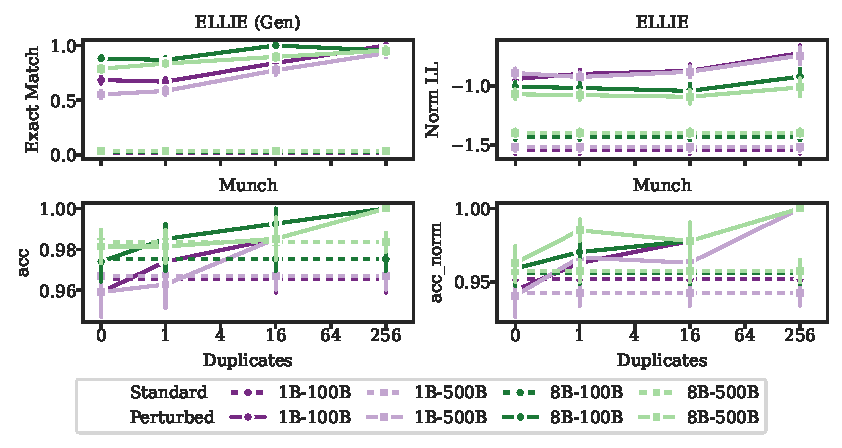
\includegraphics[width=\textwidth]{figures/domain-specific/testset-set2.pdf}
    \caption{\textbf{Core results on ELLie and MUNCH.} }
    \label{fig:testset-set2}
\end{figure}

\paragraph{MUNCH is solved by standard models.} From Figure \ref{fig:testset-set2}, we see that both standard and perturbed models achieve very high accuracy on MUNCH. Each MUNCH example consists of two sentences, one of which is the original, valid sentence, and the other is modified by swapping one word from the original sentence for an inappropriate synonym. The task is to identify which sentence is meaningful and valid. Our core models are all competent at language modeling and thus can solve the task with high accuracy ($>$ 96\%). Even so, we see increased accuracy with perturbed models on the examples that are duplicated more than 16 times.

\paragraph{ELLie examples are minimal pairs making it isolate to disentangle the effect of duplication.} ELLie is a task that tests whether language models can understand sentences with ellipsis. From Figure \ref{fig:testset-set2}, we see that the standard model achieve near 0 accuracy on the task. On the other hand, perturbed models achieve accuracy greater than 50\% even on examples that were never duplicated. On further analysis, we realized that the examples in ELLie are minimal pairs.\footnote{Many examples in ELLie contain the same first sentence but different query sentences (the second sentence). Thus, they passed our deduplication check.} When we insert the examples in our corpus, examples with the same first sentence were put in different duplication bins, e.g., of all the examples with the same core sentence, some examples were sometimes duplicated 0 times and other examples were duplicated 16 times. Thus, we see that models achieve high accuracy on examples duplicated 0 times. This invalidates the use of ELLie for studying dilution.

\begin{figure}[h]
    \centering
    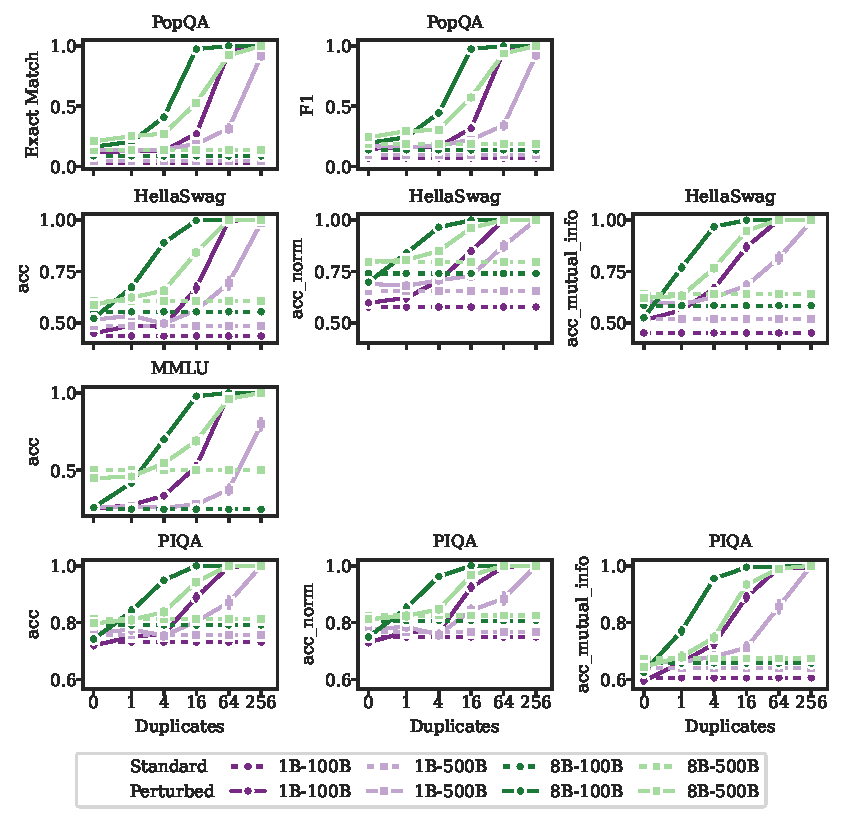
\includegraphics[width=\textwidth]{figures/domain-specific/testset-set1.pdf}
    \caption{\textbf{Core results on Test Sets (Part 1).} Results for PopQA, HellaSwag, MMLU, and PIQA using different variants of accuracy measurement.}
    \label{fig:testset-set1}
\end{figure}

\begin{figure}[h]
    \centering
    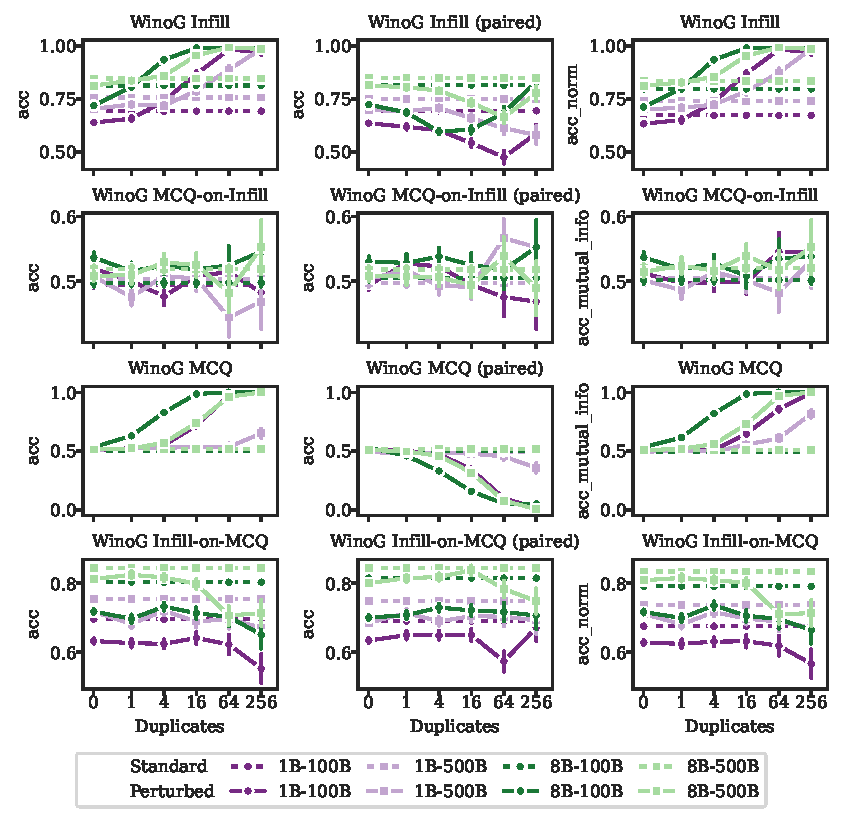
\includegraphics[width=\textwidth]{figures/domain-specific/testset-wg.pdf}
    \caption{\textbf{Core results and variants on WinoGrande.} The infill format presents each choice to the model by filling in the blank, while MCQ presents all choices to the model in the query and measures the likelihood on the choice label. Rows 1 and 2 evaluate accuracy on duplications \textit{inserted} with the Infill format. Rows 3 and 4 evaluate accuracy on duplications \textit{inserted} with the MCQ format. Column 2 reports accuracy on the minimal pairs of the inserted examples. Rows 1 and 4 use the Infill format for evaluation while rows 2 and 3 use the MCQ format for evaluation.}
    \label{fig:testset-wg}
\end{figure}

~\newpage
~\newpage
\section{Additional Results}
\label{app:additional_results}

\subsection{Timing Runs}
\label{app:timing_results}

To study how memorization evolves over training, we evaluate memorization on intermediate checkpoints every 2,000 steps up to 48,000. We also include Timing runs to analyze forgetting. Figure \ref{fig:checkpoint-forgetting-curves} reports normalized log-likelihood on Wikipedia passages and accuracy on MRPC paraphrases, each inserted 256 times. Across all four Timing runs, both metrics rise as duplicated data are encountered, peak once all perturbations have been seen, and then decay.

% \subsection{Temporal Effects}

\begin{figure}[h]
    \centering
    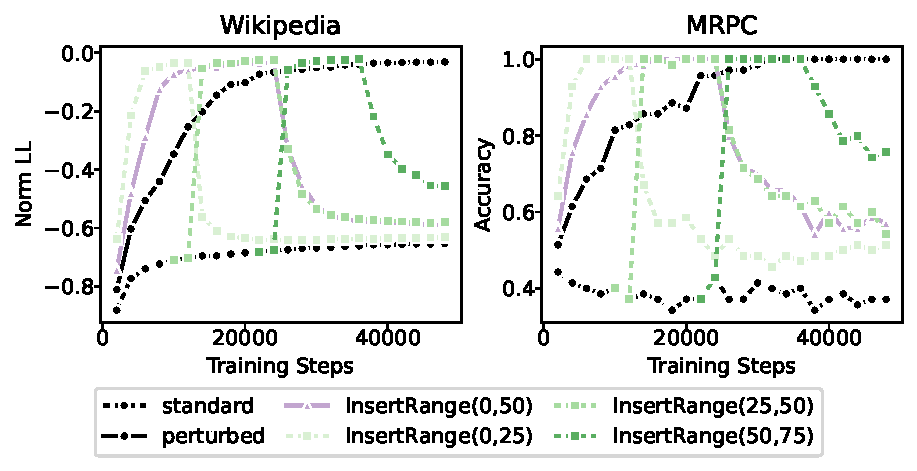
\includegraphics[width=\textwidth]{figures/injectrange/checkpoint-forgetting-curves.pdf}
    \caption{\textbf{Forgetting curves for the intermediate checkpoints of Timing runs.} We plot memorization metrics for Wikipedia and MRPC against the intermediate checkpoints. We report results on the subset of examples duplicated 256 times. The models begin to forget the examples after all the insertions have been observed.}
    \label{fig:checkpoint-forgetting-curves}
\end{figure}

\begin{figure}[h]
    \centering
    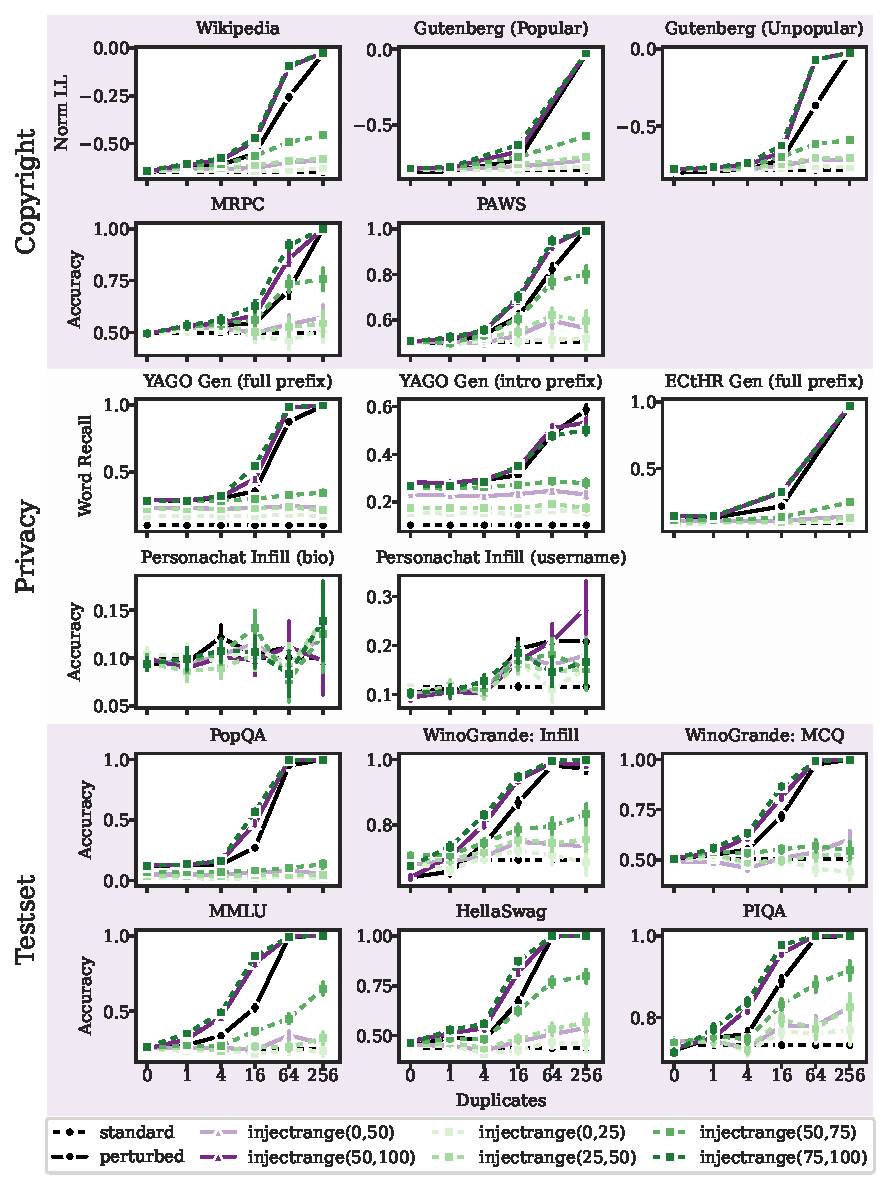
\includegraphics[width=\textwidth]{figures/injectrange/injectrange-full.pdf}
    \caption{\textbf{Evaluation on the InsertRange models.} Models that were trained on perturbations only in the early stages of training have lower performance on the memorization tasks than models trained on perturbations in the late stages of training. \texttt{InsertRange(x,y)} denotes a model trained on a corpus with perturbations inserted in batches between x\% and y\% of training.}
    \label{fig:injectrange-full}
\end{figure}
\clearpage

\subsection{Paraphrased Runs}
\label{app:paraphrase_results}

\begin{figure}[h]
    \centering
    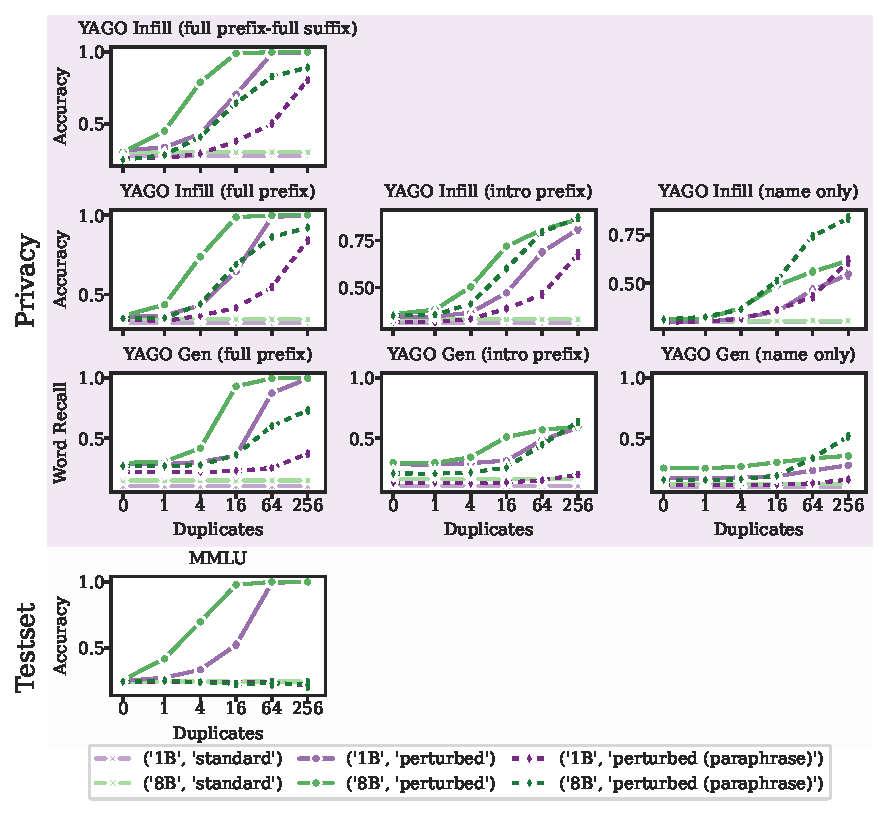
\includegraphics[width=\textwidth]{figures/paraphrase/paraphrase-full.pdf}
    \caption{\textbf{Performance of Hubble perturbed models trained on paraphased insertions.} The models do not generalize from paraphrased examples seen in training to the original examples. However, PII can be reconstructed from models trained on paraphrased biographies, even with stronger attacks.}
    \label{fig:paraphrase-full}
\end{figure}

\textbf{Data Preparation for Paraphrase Runs.} We construct paraphrased variants of the YAGO biographies and MMLU test set with \texttt{gpt-4.1-mini}. Unless otherwise noted, generation uses \texttt{temperature=1} and \texttt{top\_p=1}.
For each original perturbation example to be inserted, we obtain as many paraphrases as its required duplication count.

\begin{itemize}
    \item \textbf{MMLU paraphrases.} We follow the paraphrasing instruction of \citet{mmlu_paraphrase}. When a paraphrase query is declined by \texttt{gpt-4.1-mini} API's safety filter, we use \texttt{gemini-2.5-flash-lite} with the same parameters. 
    
    \item \textbf{YAGO paraphrases.} We adopt the diverse-style watermarking generation instructions from \citet{yago_paraphrase}. Each paraphrase is checked with a string-matching validator to ensure all biographical attributes are preserved. A paraphrase is accepted only if every attribute appears. We follow the procedure until we obtain the required number of valid paraphrases.
\end{itemize}

We train two perturbed models (1B and 8B parameters) on 100B tokens with the same perturbation data as the core perturbed model but with two data sets paraphrased: MMLU and YAGO Biographies. We evaluate the behavior of the `paraphrase' models on MMLU and YAGO evaluations in Figure \ref{fig:paraphrase-full}.

\textbf{PII can be leaked from paraphrased biographies with loss-based choice and generative evaluations.} The weakest attacks, which assume that the attacker has access to all PII about a person except one fact, are successful on models trained with paraphrased biographies. However, they have lower effectiveness than extracting the facts from the model that was trained on the original biographies. PII can be extracted with 100\% accuracy from the core 8B perturbed model using the full prefix and full suffix MCQ format. This accuracy drops to 89\% when extracting PII from the paraphrase model. Surprisingly, when using stronger attacks (attacker has access to only the persons name), PII is more accurately extractable from the 8B model trained on paraphrased biographies compared to the core models. However, this finding depends on the format of the attack and scale; generative evaluations cannot extract PII from the 1B paraphrased model. 

\textbf{Models cannot generalize from paraphrased MMLU to the original examples.} We find that both models (1B and 8B parameters) obtain random accuracy on the MMLU MCQ evaluations when trained on paraphrased versions of the examples. 

\newpage
\subsection{Architecture Runs}
\label{app:architecture_results}

\begin{figure}[h]
    \centering
    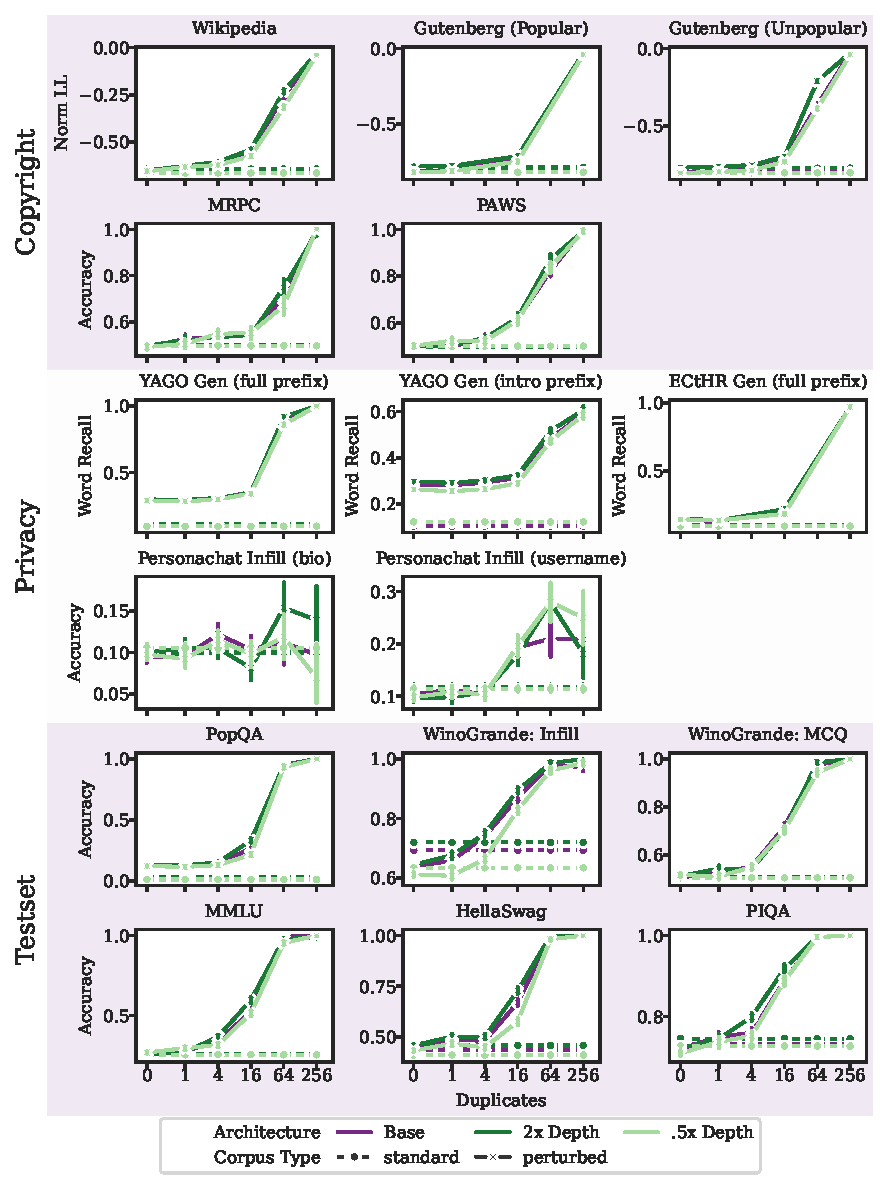
\includegraphics[width=\textwidth]{figures/architecture/architecture-full.pdf}
    \caption{Deeper models memorize slightly more than shallower models. We train three 1B-parameter models with 8, 16, and 32 layers, adjusting width to keep total parameters constant ($\approx1.2$B). All models are pre-trained on 100B tokens. As shown in Figure \ref{fig:architecture-full}, the deeper (narrower) model memorizes slightly more than the base 16-layer model, while the shallower (wider) model memorizes less.}
    \label{fig:architecture-full}
\end{figure}


